\chapter{Additional experiments results}
\label{app:experiments}

In this appendix we present and discuss additional material supporting the experiments in chapter \ref{chap:experiments}. First we present an additional visualization of the water treatment plant data in section \ref{sec:app_visualization}. In section \ref{sec:app_results_unscaled} we present the results corresponding to the experiments with the unstandardized non-temporal data sets.

\section{Visualization of water treatment plant data}
\label{sec:app_visualization}

Figure \ref{fig:experiments_swat_scatter} shows all the pairwise scatter plots of the time series $\mathbf{x}_j$ versus $\mathbf{x}_k$ from the water treatment plant data. This plot therefore shows the data points in a feature space leaving the time component aside. The normal data points are plotted in black and the outliers in red. The diagonal shows the univariate distribution of each time series $\mathbf{x}_j$ separately. 

\begin{figure}[h]
	\centering
	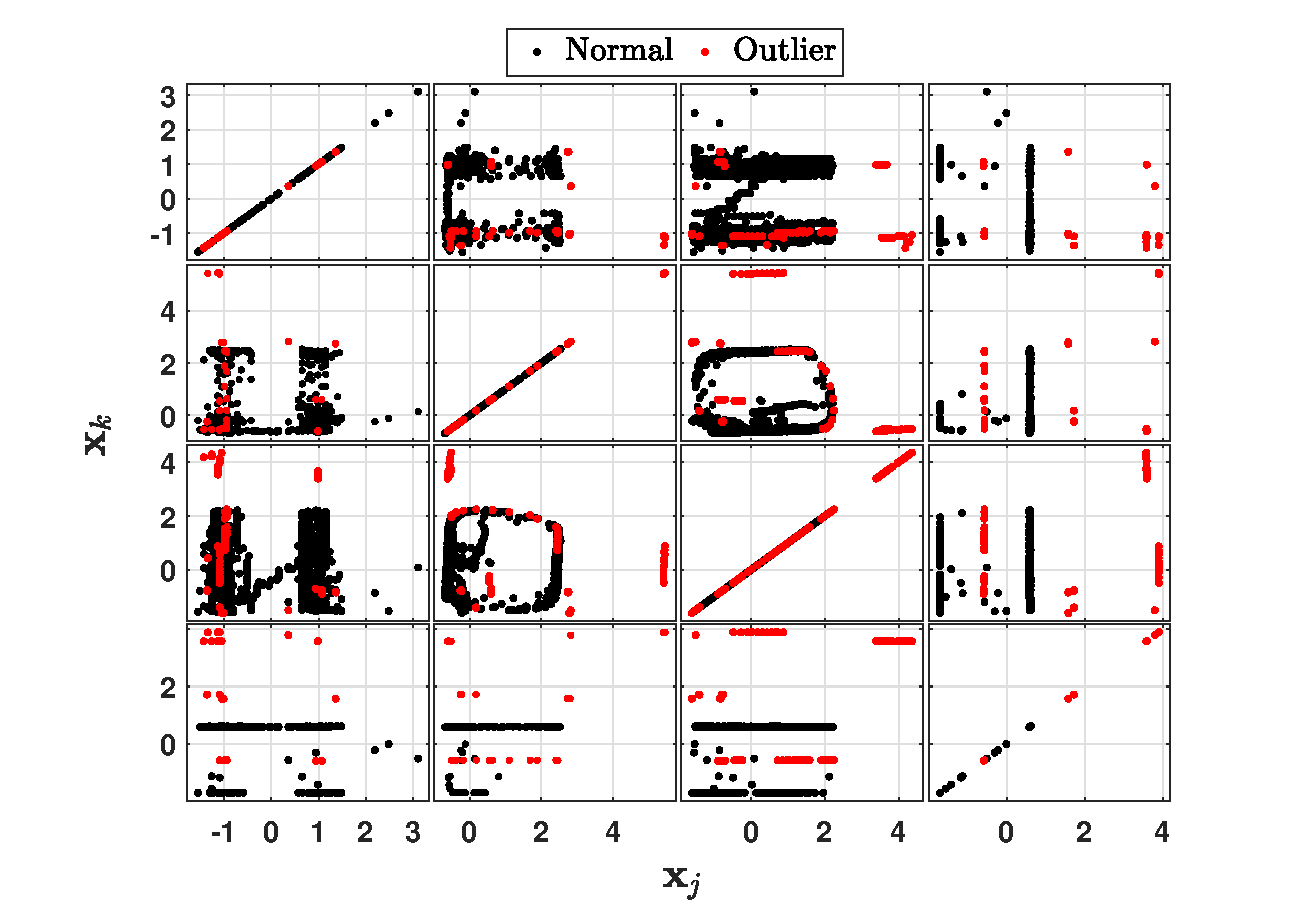
\includegraphics[scale=0.65]{experiments/Scattermatrix_swat_timeseries}
	\caption{Pairwise scatter matrix with normal data points (black) and outliers (red).}
	\label{fig:experiments_swat_scatter}
\end{figure}

Clearly, the red points that are not close to any black points correspond to the global outliers. Red points surrounded with black points correspond to the contextual outliers.

\section{Results with unstandardized non-temporal data sets}
\label{sec:app_results_unscaled}

Table \ref{tab:experiments_stand_nontemporal} presents the results obtained with the RP and $\Delta$RP method on the unstandardized non-temporal benchmark data sets as used in section \ref{sec:experiments_beyond}. In this table we only replaced the results of the RP and $\Delta$RP method as no information about the deployed preprocessing procedure for the LOF method was available and we already know PCA heavily relies on the range of the data. For the sake of easy comparison, we also provide the table with standardized data in table \ref{tab:experiments_nontemporal} as already presented in section \ref{sec:experiments_beyond}. All results were averaged over $50$ runs with distinct random projection matrices. Results that are significantly better than the opponent(s) according to the \textit{t}-statistic are made bold. 

\begin{table}[h]
	\centering
	\small
	\caption{Detection performances on \textit{unstandardized} non-temporal data.}
	\label{tab:experiments_nontemporal}
	\begin{tabular}{l c c c c}
		\toprule	
		\multirow{2}{*}{\textbf{Dataset}} & \multicolumn{4}{c}{\textbf{AUC}} \\
		\cmidrule{2-5}
					& \textbf{RP} 				& \textbf{$\Delta$RP} 			&  \textbf{PCA}		& \textbf{LOF}	\\
		\midrule
		Mammography & $\mathbf{0.89 (\pm 0.01)}$& $0.87 (\pm 0.03)$				& $0.76$			& $0.67$  	\\
		Thyroid (Ann-)  & $0.54 (\pm 0.01)$ 	& $0.62 (\pm 0.03)$ 			& $0.49$			& $\mathbf{0.72}$	\\
		Pima 		& $0.71 (\pm 0.02)$ 		& $\mathbf{0.77 (\pm 0.01)}$ 	& $0.57$			& $0.49$	\\	
		BCW\footnote{BCW refers to the Breast Cancer Wisconsin data set}	& $\mathbf{1.00 (\pm 0.00)}$& $0.99 (\pm 0.00)$ 			& $0.89$			& $0.37$	\\
		Arrhythmia	& $0.57 (\pm 0.00)$ 		& $\mathbf{0.73 (\pm 0.03)}$  	& $0.63$			& $\mathbf{0.73}$	\\
		Ionosphere	& $0.58 (\pm 0.01)$ 		& $0.69 (\pm 0.01)$  			& $\mathbf{0.95}$	& $0.89$	\\
		\bottomrule
	\end{tabular}
\end{table}


\begin{table}[h]
	\centering
	\small
	\caption{Detection performances on \textit{standardized} non-temporal data.}
	\label{tab:experiments_stand_nontemporal}
	\begin{tabular}{l c c c c}
		\toprule	
		\multirow{2}{*}{\textbf{Dataset}} & \multicolumn{4}{c}{\textbf{AUC}} \\
		\cmidrule{2-5}
		& \textbf{RP} 			& \textbf{$\Delta$RP} 							&  \textbf{PCA}		& \textbf{LOF}	\\
		\midrule
		Mammography & $\mathbf{0.88 (\pm 0.02)}$& $\mathbf{0.88 (\pm 0.01)}$	& $0.76$			& $0.67$  	\\
		Thyroid (Ann-) & $0.67 (\pm 0.00)$ 		& $0.64 (\pm 0.02)$ 			& $0.49$			& $\mathbf{0.72}$	\\
		Pima 		& $\mathbf{0.65 (\pm 0.01)}$ & $\mathbf{0.65 (\pm 0.01)}$ 	& $0.57$			& $0.49$	\\	
		BCW  	& $0.95 (\pm 0.01)$& $\mathbf{0.97 (\pm 0.01)}$ 			& $0.89$			& $0.37$	\\
		Arrhythmia	& $\mathbf{0.77 (\pm 0.00)}$ 		& $0.75 (\pm 0.02)$  	& $0.63$			& $0.73$	\\
		Ionosphere	& $0.79 (\pm 0.00)$ 		& $0.80 (\pm 0.02)$  			& $\mathbf{0.95}$	& $0.89$	\\
		\bottomrule
	\end{tabular}
\end{table}

These two tables show large differences between the AUC's on unstandardized (table \ref{tab:experiments_nontemporal}) and standardized data (table \ref{tab:experiments_stand_nontemporal}). This likely is the consequence of the original (unstandardized) data which is not close to having $0$ mean and unit variance, which was the case for the synthetic data in the analysis. Concerning the Mammography and BCW data sets, the detection performances of the RP method and $\Delta$RP are quite similar. When we look at Thyroid (Ann-), Arrhythmia and Ionosphere we can see how the RP method is more sensitive to the range and mean of the data, as its AUC drops significantly when the data is unstandardized. More specifically, the AUC of the RP method drops from $0.67$ to $0.54$ on Thyroid, from $0.77$ to $0.57$ on Arrhythmia, and from $0.79$ to $0.58$ on Ionosphere, while we observe smaller differences in AUC for $\Delta$RP. For the Pima data set both methods perform significantly better when the data is left unstandardized. Going from these observations, we can say that $\Delta$RP is less sensitive to the range and mean of the data than the RP method. 
